% \newpage
\section{Reproducibility Summary}

\subsection*{Scope of Reproducibility}
% State the main claim(s) of the original paper you are trying to reproduce (typically the main claim(s) of the paper).
% This is meant to place the work in context, and to tell a reader the objective of the reproduction.
\citeauthor{gao2021privacy} \cite{gao2021privacy} propose to leverage policies consisting of a series of data augmentations for preventing the possibility of reconstruction attacks on the training data of gradients. The goal of this study is to: (1) Verify the findings of the authors about the performance of the found policies and the correlation between the reconstruction metric and provided protection. (2) Explore if the defence generalizes to an attacker that has knowledge about the policy used.

\subsection*{Methodology}
% Briefly describe what you did and which resources you used. For example, did you use author's code? Did you re-implement parts of the pipeline? You can also use this space to list the hardware used, and the total budget (e.g. GPU hours) for the experiments. 
For the experiments conducted in this research, parts of the code from \citeauthor{gao2021privacy} were refactored to allow for more clear and robust experimentation. Approximately a week of computation time is needed for our experiments on a 1080 Ti GPU.

\subsection*{Results}
It was possible to verify the results from the original paper within a reasonable margin of error. However, the reproduced results show that the claimed protection does not generalize to an attacker that has knowledge over the augmentations used. Additionally, the results show that the optimal augmentations are often predictable since the policies found by the proposed search algorithm mostly consist of the augmentations that perform best individually.


\subsection*{What Was Easy}
% Describe which parts of your reproduction study were easy. For example, was it easy to run the author's code, or easy to re-implement their method based on the description in the paper? The goal of this section is to summarize to a reader which parts of the original paper they could easily apply to their problem.
The design of the search algorithm allowed for easy iterations of experiments since obtaining the metrics of a single policy can be done in under a minute on an average GPU. It was helpful that the authors provided the code of their experiments.

\subsection*{What Was difficult}
% Describe which parts of your reproduction study were difficult or took much more time than you expected. Perhaps the data was not available and you couldn't verify some experiments, or the author's code was broken and had to be debugged first. Or, perhaps some experiments just take too much time/resources to run and you couldn't verify them. The purpose of this section is to indicate to the reader which parts of the original paper are either difficult to re-use, or require a significant amount of work and resources to verify.
To obtain the reconstruction score and accuracy of a policy, the architecture needs to be trained for about 10 GPU-hours. This makes it difficult to verify how well the search metrics correlate with these scores. It also prevented us to test the random policy baseline, as this requires the training to be repeated at least 10 times which requires significant computational power.

\subsection*{Communication With Original Authors}
% Briefly describe how much contact you had with the original authors (if any).
An e-mail was sent to the original authors regarding the differences in results. Unfortunately no response has been received so far.

% \subsection{Submission Checklist}

% Double check the file \texttt{journal/metadata.yaml} to contain the following information:

% \begin{itemize}
% \item Title should start with "\texttt{[Re]}"
% \item Author information, along with ORCID id
% \item Author affiliations
% \item Code URL, Software Heritage Foundation link
% \item Abstract
% \item Review URL (the OpenReview URL of your report)
% \end{itemize}

% \subsection{Continuous Integration}

% We use Github Actions CI to check your submission and compile the pdf file subsequently.
% You can also run the tests locally by running \texttt{python check\_yaml.py}, and then running \texttt{./build.sh} to compile Latex.

\clearpage

% \section{Content}

\newpage
% The following section formatting is optional you can also define sections as you deem fit. Focus on what future researchers or practitioners would find useful for reproducing or building upon the paper you choose.


\section{Introduction}
Collaborative learning is becoming increasingly common. A deep learning model can be trained by multiple participants without the parties having to share their training set  \cite{yang2019federated, guo2020towards, melis2019exploiting}. Instead, they share gradients, given a public model. This allows private data to be used for training non-private networks. However, recent works discovered that the shared gradients may be used to recover sensitive training samples. This development poses a serious threat to collaborative learning. \citeauthor{gao2021privacy}\cite{gao2021privacy} proposes the ATSPrivacy-Framework as a solution for such reconstruction attacks.

The goal of the ATSPrivacy-Framework is to use simple data augmentations, such as translations and changes in contrast, to obfuscate the images and make them more difficult to reconstruct. The authors show that some of these augmentations significantly increase privacy under their attack model without severely impacting the accuracy. A search algorithm is designed to find a combination of augmentations (referred to as a \textit{policy}) that work well. The search algorithm aims to find the policy that protects the privacy of training images the most, while still maintaining model accuracy. A \textit{privacy score} and an \textit{accuracy score} are introduced as search metrics in order to estimate the reconstruction score of an attacker and the accuracy of the model. The accuracy score is implemented based on techniques from \citeauthor{mellor2021neural} \cite{mellor2021neural}, and the privacy metric is a novel technique. The authors claim that the metrics provide suitable estimations of the model accuracy and reconstruction score, without needing to train the model first.

As a response on \citeauthor{gao2021privacy}, \citeauthor{balunovic2021bayesian} \cite{balunovic2021bayesian} have shown that the proposed method is not secure during early stages of training. The goal of this research is to extend the research of \citeauthor{gao2021privacy}, and find out whether the method is also insecure in the final stages of training. This will be researched by incorporating knowledge of the policies being used as a defense into the attack model.

% For this reason we test a modified attack model where the attacker learns a translation along with the reconstruction of an image and we evaluate whether the privacy improvements still hold under this model.


\section{Scope of Reproducibility}
\label{sec:claims}

% Introduce the specific setting or problem addressed in this work, and list the main claims from the original paper. Think of this as writing out the main contributions of the original paper. Each claim should be relatively concise; some papers may not clearly list their claims, and one must formulate them in terms of the presented experiments. (For those familiar, these claims are roughly the scientific hypotheses evaluated in the original work.)

% A claim should be something that can be supported or rejected by your data. An example is, ``Finetuning pretrained BERT on dataset X will have higher accuracy than an LSTM trained with GloVe embeddings.''
% This is concise, and is something that can be supported by experiments.
% An example of a claim that is too vague, which can't be supported by experiments, is ``Contextual embedding models have shown strong performance on a number of tasks. We will run experiments evaluating two types of contextual embedding models on datasets X, Y, and Z."

% This section roughly tells a reader what to expect in the rest of the report. Clearly itemize the claims you are testing:
% \begin{itemize}
%     \item Claim 1
%     \item Claim 2
%     \item Claim 3
% \end{itemize}

% Each experiment in Section~\ref{sec:results} will support (at least) one of these claims, so a reader of your report should be able to separately understand the \emph{claims} and the \emph{evidence} that supports them.
The reproducibility is split into two parts. The aim of the first part is to reproduce the claims from \citeauthor{gao2021privacy}, by recreating their experiments. The second part of this research focusses on the expansion of the original framework by performing additional experiments that give insight in how the findings of the authors are able to generalize to more intelligent attackers.

\subsection{Reproduction}
The first results are generated to reproduce the correlation between the proposed privacy score as an estimation of the reconstruction score after training. This will be done by recreating the empirical validation mentioned in the paper of \citeauthor{gao2021privacy}. This work will not include experiments on researching the accuracy score, as the authors base this decision on previous work and this experiment would require a lot of computing power than available. Additionally, the performance of the policies found by the authors is verified using the search algorithm created by \citeauthor{gao2021privacy}.
% This is done by training models on the different policies and comparing their performance to the scores without an augmentation policy.
Concretely, the two claims that are reproduced are:
\begin{enumerate}
    \item The privacy score proposed in the paper correlates with the reconstruction score of an attack.
    \item The policies selected by the search algorithm reduce the reconstruction score significantly while not resulting in a great loss of accuracy.
\end{enumerate}

\subsection{Additional Insight}
In the original paper several attack methods have been tested, which all follow the same strategy but with different optimizers and distance measures. This is further illustrated in Section \ref{sec:method}. All the attack methods do not use any knowledge about possible augmentations on the data. The goal of this study is to provide insight into what happens when an attacker makes assumptions on what augmentations are used. Additionally, this claim is supported by showing that the policies that are found by the model have very limited diversity, which makes it easy to predict what augmentations are used. This research provides the following insights:
\begin{enumerate}
    \item The effectiveness of the most promising policies selected by the paper for protecting the data is greatly reduced when the attacker knows that this policy is being used.
    \item Most policies score worse than no policy on both the accuracy and privacy search metric.
    \item The policies that score better than no policy on the search metrics often consist of the augmentations that scored best individually.
\end{enumerate}

%\jdcomment{To organizers: I asked my students to connect the main claims and the experiments that supported them. For example, in this list above they could have ``Claim 1, which is supported by Experiment 1 in Figure 1.'' The benefit was that this caused the students to think about what their experiments were showing (as opposed to blindly rerunning each experiment and not considering how it fit into the overall story), but honestly it seemed hard for the students to understand what I was asking for.}


\section{Methodology} \label{sec:method}
% Explain your approach - did you use the author's code, or did you aim to re-implement the approach from the description in the paper? Summarize the resources (code, documentation, GPUs) that you used.

\subsection{Model Descriptions}
% Include a description of each model or algorithm used. Be sure to list the type of model, the number of parameters, and other relevant info (e.g. if it's pretrained). 
Two models are used in the framework, the system and attack models. The system model is a standard collaborative learning system where multiple parties train a global model \textit{M}. The Attack model is considered an independent party in the collaborative learning system. The gradients are shared to all parties in each iteration and the attacker tries to reconstruct private training samples from the shared gradients.

\textbf{System Model}
Multiple parties train a global model \textit{M}. All participants own a private dataset \textit{D}. Let $\mathcal{L}$ be the loss function and let \textit{W} bet the model parameters. Each iteration a training sample $(x,y)$ is randomly selected by all parties. After randomly selecting the training sample, the loss $\mathcal{L}(x,y)$ is calculated using forward propagation and then the gradient $\nabla W(x,y) = \frac{\partial \mathcal{L}(x,y)}{\partial W}$ is calculated using backpropagation.

% The system models is a collaborative learning model where multiple parties train a global model \textit{M}. All participants own a dataset \textit{D}. This dataset is private and is not shared with the other participants. Let $\mathcal{L}$ be the loss function and let \textit{W} bet the model parameters. Each iteration a training sample $(x,y)$ is randomly selected by all parties. After randomly selecting the training sample, the loss $\mathcal{L}(x,y)$ is calculated using forward propagation, after this the gradient $\nabla W(x,y) = \frac{\partial \mathcal{L}(x,y)}{\partial W}$ is calculated using back propagation. 

\textbf{Attack Model}
Given a gradient $\nabla W(x,y)$ the attacker wants to find a sample and label pair $(x',y')$, such that the matching gradient $\nabla W(x',y')$ approximates $\nabla W$. This can be expressed by minimizing the optimization problem shown in Equation \ref{eq:1}.
% The original attack model used in the paper tries to reconstruct private training samples using the gradients received in each iteration. Different optimization algorithms are used to extract information from the gradients. Given a gradient $\nabla W(x,y)$ the attacker wants to find a sample and label pair $(x',y')$, such that the matching gradient $\nabla W(x',y')$ approximates $\nabla W$. This can be expressed by minimizing the optimization problem shown in equation \ref{eq:1}. 

\begin{equation}
    \label{eq:1}
    x^*,y^* = argmin_{x',y'} ||\nabla W(x,y) - \nabla W(x',y')||
\end{equation}

A reconstruction attack is considered successful when $x^*$ is very similar to $x$. The term $||\nabla W(x,y) - \nabla W(x',y')||$ is called the gradient loss. This term corresponds with the L1-norm, but it can also be replaced by the L2-norm or cosine distance.

\textbf{Protection}
In order to protect against reconstruction attacks the original dataset $D$ is transformed into a new dataset $\hat{D}$. The new dataset is created by applying a set of transformation functions $T = t_1 \circ t_2 \circ ... \circ t_n$ on each sample $x \in D$, resulting in $\hat{x} = T(x)$. The data owner then uses $\hat{D}$ to calculate the gradients during training and shares them with the other participants.
% In order to protect against reconstruction attacks the original dataset $D$ is transformed into a new dataset $\hat{D}$. The new dataset is created by applying a set of transformation functions $T = t_1 \circ t_2 \circ ... \circ t_n$ on each sample $x \in D$, resulting in $\hat{x} = T(x)$. The data owner can use $\hat{D}$ to calculate the gradients and share them with the other participants without the risk of reconstruction. There are two requirements for a transformation policy: 1) An attacker should not be able to reconstruct $\hat{x}$ (and x) from $\nabla W(\hat{x}, y)$. 2) The new model should have similar performance to the original model. 

\textbf{Privacy Score} Due to the expensive computation time of the PSNR metric, it is not an efficient method to compare the privacy effect amongst candidate policies. A new privacy score is developed by the authors, which is intended to reflect the privacy leakage given a transformation policy and a model which is trained only for a few epochs. The privacy score is given by Equation \ref{eq:spri}. This equation is a numerical integration over $K$ steps which estimates the area under the curve of the gradient similarity during a reconstruction attack.

\begin{equation}
    \label{eq:spri}
    S_{pri} (T) \approx \frac{1}{|D| K} \sum_{x\in D}\sum_{j=0}^{K-1} \texttt{GradSim} (x'(\frac{i}K),T(x))
\end{equation}


Where $x'(i) = (1 - i) * x_0 + i * T(x)$ and \texttt{GradSim} measures the gradient similarity between two input samples $(x_1, x_2)$ with the same class $y$, as given by equation \ref{eq:gradsim}.

\begin{equation}
    \label{eq:gradsim}
    \texttt{GradSim}(x_1,x_2) = \frac{<\nabla W(x_1, y), \nabla (x_2, y)>}{|| \nabla W(x_1,y)|| \cdot ||\nabla W(x_2,y)||}
\end{equation}

% Let the transformed image be $\hat{x}$. When an attacker tries to reconstruct $\hat{x}$, the attacker starts from a random input $x' = x_0$, and updates $x'$ iteratively using equation \ref{eq:1}. This updates converges when $\nabla W(x', y)$ approaches $\nabla W(\hat{x}, y)$

\textbf{Accuracy Score}
Besides the privacy requirement, it is also important to maintain model accuracy. \citeauthor{mellor2021neural} \cite{mellor2021neural} proposed a technique to explore neural architectures without the need of model training. Based on this work \citeauthor{gao2021privacy} create a technique to search for transformations that maintain model performance. The accuracy score defined by \citeauthor{gao2021privacy} is shown in Equation \ref{sacc}.
% Besides the privacy requirement, it is also important to maintain model accuracy. Joseph et al. \cite{} proposed a technique to explore neural architectures without the need of model training. This method empirically evaluates the correlations between the local linear map and architecture performance. The maps that yield the best performance are then identified by this method. Based on this work Wei Gao et al. create a technique to search for transformations that maintain model performance. Let's initialize a random model $f$, and create a mini-batch of data samples that is transformed by the target policy $T: \{\hat{x_n\}^N_{n=1}}$. First the Gradient Jacobian matrix is calculated as shown in figure \ref{eq:3} below. 

% \begin{equation}
%     \label{eq:3}
%     J = (\frac{\partial f}{\partial \hat{x}_1}, \frac{\partial f}{\partial \hat{x}_2}, ..., \frac{\partial f}{\partial \hat{x}_N})^T
% \end{equation}

% Using the Jacobian matrix, the correlation matrix can be calculation:

% \begin{equation}
%     \label{eq:4}
%     (M_J)_{i,j} = \frac{1}{N} \sum^N_{n=1} J_{i,j} 
% \end{equation}
% \begin{equation}
%     C_J=(J-M_J)(J-M_J)^T
% \end{equation}

% \begin{equation}
%     \label{eq:5}
%     (\Sigma_J)_{i,j} = \frac{(C_J)_{i,j}}{\sqrt{(C_J)_{i,i} \cdot (C_J)_{j,j}}}
% \end{equation}

% Let $\sigma_{J,1} \leq ... \leq_{J,N}$ be the \textit{N} eigenvalues of $\Sigma_J$, then the accuracy score can be defined as:

\begin{equation}
    \label{sacc}
    S_{acc}(T) = \frac{1}{N} \sum^{N-1}_{i=0} \log(\sigma_{J,i} + \epsilon) + (\sigma_{J,i} + \epsilon)^{-1}
\end{equation}

Where $\epsilon$ is a small positive value used for numerical stability, and $\sigma_{J,i}$ is the $i$'th eigenvalue of the correlation matrix of the jacobian $J=(\frac{\partial f}{\partial \hat x_1}, \dotso \frac{\partial f}{\partial \hat x_N})$ for a randomly initialized model $f$ and a mini-batch of samples transformed by the target policy $T: \{ \hat x_n \}_{n=1}^N$.

% \textbf{Finding and Adopting Transformations}
% $\epsilon$ is set to $10^{-5}$ in order to achieve numerical stability. The accuracy score defined above are utilized to find the best policies, and apply them to collaborative training. The AutoAugment \cite{} augmentation library containing 50 distinct transformation functions is used to find suitable policies. At most \textit{k} functions are combined in a policy. This results in a search space of $\Sum^K_{i=1} 50^i$ policies. Only $C_{max}$ policies are tested. In this research we use $K=3$ this results in a search space of 127550. We set $C_max$ to 1500, this should be large enough to find qualified policies.

\textbf{The Search Algorithm}
The goal of the search algorithm is to identify a policy set by combining qualified methods. Two models should be prepared: (1) the privacy quantification model, (2) a model that is randomly initialized without the use of any optimization strategies. This second model is used for accuracy quantification. $C_{max}$ policies are randomly sampled. The privacy and accuracy scores of each policy are then calculated. When the accuracy score is lower than a predefined threshold, the policy is rejected. The top-$n$ polices are then selected based on the privacy score from the final policy set.
% The algorithm defined below shows the search process used in the research of Wei Gao et al.. The goal is to identify a policy set $\tau$ using $n$ qualified methods. Two models should be prepared: (1) $M^s$ is used for privacy quantification. (2) $M^r$ is a model that is randomly initialized without the use of any optimization strategies. This second model is used for accuracy quantification. $C_{max}$ policies are randomly sampled. The privacy and accuracy scores of each policy are then calculated. When the accuracy score is lower than a threshold $\tau_{acc}$, the policy is rejected. The top-$n$ polices are then selected based on the privacy score from the final policy set $\tau$. 

% \begin{algorithm}[H]
% \SetAlgoLined
% \KwData{Augmentation library P, $T_{acc}$, $C_{max}$, $M^s$}
% \KwResult{Optimal policy set $\tau$ containing n policies }
%  \While{i \in [1, C_max}{
%   Sample functions from P to form a policy T\;
%   Calculate S_{acc}(T) from M^r, D\;

%   \If{S_{acc} \geq T_{acc}}
%   {\eIf{|\tau| < n}{
%   Insert T to \tau\;
%   }{
%   Calculate S_{pri}(T) from M^s, D\;
%   T^* \leftarrow argmax_{T' \in $\tau$}S_{pri}(T')\;
%   \If{S_{pri}(T) < S_{pri}(T^*)}
%   {Replace T^* with T in $\tau$}
%   }}
%   \If{|$\tau$| < n}{Go to Line 1;}
%   \textbf{Return} $\tau$
%  }
%  \caption{Searching for optimal transformations}
% \end{algorithm}
% \includegraphics[scale=.5]{Screenshot from 2022-01-23 19-16-58.jpg}


% \textbf{The Application of Transformations} Given the policy set $\tau$ we just found, the function's can be applied over the sensitive training data. One approach is to always select the policy with the smallest $S_{pri}$, and then apply this to each sample. However, a single fixed policy can affect domain shifts and bias in the in input samples. This can affect the performance, although this was tested using the accuracy metric. To prevent this a hybrid augmentation strategy is used. A transformation policy from $\tau$ is randomly selected. The selected policies cannot have transformation functions in common. This guarantees low privacy leakage and high model accuracy. This can also improve model generalization and domain shifts.

\textbf{Enhanced Attack Model}
It can be expected that an attacker has knowledge about the augmentations that are used to protect the data. Based on this assumption, a simple variation on the attack model is explored that allows the attacker to learn a translation along with the reconstruction of an image. This is inspired by the observation that all the successful augmentations selected by the paper make use of translations or crops that create large black areas in the image, but the original reconstruction algorithm is never able to reconstruct these.

In order to learn this translation, the attempted solution $x*$ which is being reconstructed by the algorithm is first put through a translation module. This module can be fine-tuned during the reconstruction process by the attacker in order to find a suitable translation that reduces the gradient loss. This is done by propagating the gradients through the differentiable translation module and training the parameters $t_x$ and $t_y$, denoting the shift of the image on the $x$ and $y$ axes respectively. A more general affine transformation can also be learned, but this is of little use for the given augmentations since they don't shear, scale or rotate the images. The implementation of this translation module is inspired by Spatial Transformer Networks \cite{jaderberg2015spatial} which use a similar mechanism to preprocess data before it is given to convolutional neural networks. Figure \ref{fig:enhfg} illustrates how the enhanced algorithm works.

The parameters $t_x$ and $t_y$ from the translation module are constrained to a maximum and minimum constant each such that the translation does not become too large. These constraints are set depending on the augmentation policy under attack.

\begin{figure}
    \centering
    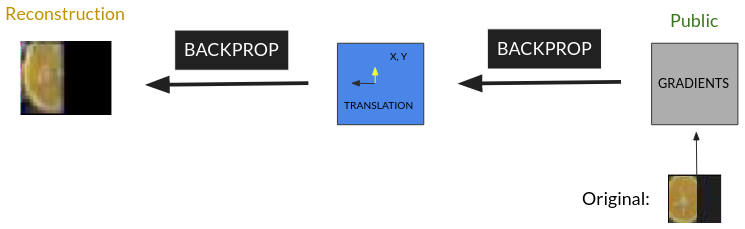
\includegraphics[width = 0.7\textwidth]{enhfig2.png}
    \caption{Enhanced attack algorithm}
    \label{fig:enhfg}
\end{figure}

% The second method is inspired by the observation that all of the successful augmentations selected by the paper make use of translations to protect the data. In particular, some of these apply a translation that either moves an image half a frame to the right, or half a frame to the left. See Figure \ref{}. This method then simply enforces that the solution is translated in the same way before it is given as input to the neural network.

\subsection{Datasets}
% For each dataset include 1) relevant statistics such as the number of examples and label distributions, 2) details of train / dev / test splits, 3) an explanation of any preprocessing done, and 4) a link to download the data (if available).
\citeauthor{gao2021privacy} used the CIFAR100 \cite{unknown-author-2009} and Fashion MNIST \cite{xiao2017fashionmnist} datasets during their research. The CIFAR100 dataset consists of 100 distinct classes, each containing 600 32x32 images. There are 500 training images and 100 testing images per class. The Fashion MNIST contains 70,000 fashion products which can be assigned to 10 distinct categories. Each of the 10 classes contains 7,000 images. There are 60,000 training images and 10,000 testing images.

% Besides these two datasets we also used the ImageNet dataset. The ImageNet dataset is structured like the WordNet hierarchy and contains 14,197,122 annotated images. The hierarchical structure of this dataset does not assign instances to classes, but rather maps the relationship between the instances. 

\subsection{Hyperparameters}
% Describe how the hyperparameter values were set. If there was a hyperparameter search done, be sure to include the range of hyperparameters searched over, the method used to search (e.g. manual search, random search, Bayesian optimization, etc.), and the best hyperparameters found. Include the number of total experiments (e.g. hyperparameter trials). You can also include all results from that search (not just the best-found results).

The same hyperparameters that were used in the paper are used for this reproduction. The search algorithm is trained using 10\% of the available training set for 50 epochs. The full training of a model is done with 100\% of the training set for 200 epochs. Both are trained with a batch size of 128 and Stochastic Gradient Descent (SGD) \cite{ruder2016overview} with weight decay and Nesterov momentum \cite{sutskever2013importance}. The learning rate is set to $0.1$ and decays with a multistep linear scheduler after epochs 75, 125 and 175 with a gamma of $0.1$. The parameter $\epsilon$ in equation \ref{sacc} is set to $10^{-5}$.

The reconstruction algorithm reconstructs one image at a time in 4800 iterations. The same optimizer is used with the same hyperparameters, but the learning rate decays after iterations $\sim 1800$, $\sim 3000$ and $\sim 4200$. Cosine distance is used as the gradient similarity metric (see Equation \ref{eq:1}). The constraints for the enhanced attack algorithm are set such that $|t_x| < 1.1$ and $|t_y| < 0.2$ for the \textit{3-1-7} policy (see Section \ref{sect:experiments}), $|t_x| < 0.4$ and $|t_y| < 0.4$ for the \textit{43-18-18} policy and such that $|t_x| < 1.1$ and $|t_y| < 0.4$ for the \textit{Hybrid} policy. A value of 1 for these constraints corresponds to half the width/height of the image frame.

% 50 transformations functions are available. At most \textit{k} functions are combined in a policy. This results in a search space of $\Sum^K_{i=1} 50^i$ policies. We use $K=3$ this results in a search space of 127550. 

% The ResNet20 model \cite{he2015deep} is trained on CIFAR100 with 200 epochs. 

% Figure \ref{fig:model performance} shows the accuracy and loss over the training sets and validation sets with and without the transformation policies. The figure shows that despite the fact that the augmented policies converge slower on the training set, the convergence speed on the validation set is the same. From this we can infer that the transformations entail negligible overhead for the training process.

% \begin{figure}[htp]
% \centering
%   \includegraphics[width=16cm]{Untitled.png}
%   \caption{Results of original authors that showcases the model performance of ResNet20 on CIFAR 100 during training process}
%   \label{fig:model performance}
% \end{figure}

% In figure \ref{fig:model performance} we see that the curve flattens between 150-200 epochs. From this flattening we can infer that the model performance will not significantly improve after more than 200 epochs. This justifies the choice to use 200 epochs for the model. If the figures from our reproduction are compared to the figureof Wei Gao et al, it is clear tath both figures show a SIMILAR/DIFFERENT trend as the authors of the paper, which (DOES NOT) justifie(S) the decision of 200 epochs. 


% The parameters stated above are similar to the parameters used by \citeauthor{gao2021privacy} are correct and stable.

\subsection{Experimental Setup and Code}\label{sect:experiments}
% Include a description of how the experiments were set up that's clear enough a reader could replicate the setup. 
% Include a description of the specific measure used to evaluate the experiments (e.g. accuracy, precision@K, BLEU score, etc.). 
% Provide a link to your code.

The codebase for the paper is available on GitHub \cite{weigithub}. This codebase was used in this study as a starting point to reproduce the claims made by \citeauthor{gao2021privacy}. The codebase was modified to run the experiments on systems available during this research and to run additional experiments. The models in the framework rely on the PyTorch library \cite{NEURIPS2019_9015}. The adapted code used for the experiments in this report can also be found on GitHub \cite{reproduced}. % ATSrefactored explained

% The SGD optimizer \cite{pmlr-v28-shamir13} with momentum, weight decay and learning decay techniques is used to have the guarantee the convergence of the model, better known as Adam \cite{kingma2014method}. 

At most 3 functions are drawn from a set of 50 transformations from the data augmentation library in the defence implementation. The functions are denoted as $i-j-k$ , where i, j and k are the indexes of the functions from the augmentation library. Note that functions can be applied multiple times within the same concatenation of policies.

% Wei Gao et al. use the following three defences to compare their defence strategy to: (1) \textit{Gaussian/Laplacian}: By the use of differential privacy to disturb the gradients with Gaussian or Laplacian noise. (2) \textit{Pruning}: Using a layer-wise pruning technique \cite{} to discard parameter gradients that have small absolute values. (3) \textit{Random augmentation}: randomly sampling 10 transformation policies in order to obtain the average result. 

The following experiments were conducted:
\begin{enumerate}
    \item To verify the claimed correlation, 100 random policies were evaluated by performing a reconstruction attack of 2500 iterations on a ResNet20 DNN on the CIFAR100 dataset.
    \item To verify the claimed results, four models were fully trained using the CIFAR100 dataset and the ResNet20 DNN: with no policy, the policies \textit{3-1-7}, \textit{43-18-18} and finally the \textit{Hybrid} policy, which randomly chooses either the \textit{3-1-7} augmentations or the \textit{43-18-18} augmentations for each image. This was repeated for the F-Mnist dataset with the same architecture, but using the policies \textit{19-15-45} and \textit{2-43-21}. Subsequently a reconstruction attack was performed using the same settings as the original authors.
    \item To give insight into the performance of the enhanced attack, the CIFAR100 models mentioned above were attacked using the enhanced reconstruction attack.
    \item To give insight into the distribution of policies, 1500 benchmarks were done using the privacy and accuracy score on the CIFAR100 dataset with the ResNet20 architecture. Additionally, all augmentations listed in the original paper were evaluated individually in the same setting.

\end{enumerate}

% % previous 3.4:
% The replication of the results of \citeauthor{gao2021privacy} can be divided into 5 steps. The adapted code was used for these experiments.
% \begin{enumerate}
%     \item Search for suitable policies, using the CIFAR100 dataset and the ResNet20 DNN.
%     \item Train four models fully, using the CIFAR100 dataset and the ResNet20 DNN with no policy, the policies \textit{3-1-7}, \textit{43-18-18} and the \textit{Hybrid} policy, which randomly chooses either the \textit{3-1-7} augmentations or the \textit{43-18-18} augmentations for each image.
%     \item Do the same for the F-Mnist dataset with the same architecture, but using the policies \textit{19-15-45} and \textit{2-43-21}.
%     \item Perform the default reconstruction attack on all the models trained.
%     \item Perform the enhanced reconstruction attack on the models trained with augmented policies on the CIFAR100 dataset.
% \end{enumerate}

Accuracy is used to measure model performance. Accuracy is defined as the ratio of correct classifications to the total number of classifications. The similarity of a reconstructed image to the original is measured by the Peak Signal to Noise Ratio (PSNR) \cite{hore2010image} of the two, which is measured in decibels and correlates to the logarithm of the mean square differences between the pixels of one image and the other. To measure the overall resistance of a model to reconstruction attacks, the average PSNR is taken over 100 reconstructions.
% This similarity is quantified with the Peak Signal-to-Noise Ratio (PSNR) metric \cite{hore2010image}. 
% After replication the results we test the generalizability of the framework to another dataset. For this we use the ImageNet dataset. This generalization can be divided into the same 5 steps as stated above. In order to make the framework work with other datasets the original framework had to be adjusted by ... 

\subsection{Computational Requirements}
% Include a description of the hardware used, such as the GPU or CPU the experiments were run on. 
% For each model, include a measure of the average runtime (e.g. average time to predict labels for a given validation set with a particular batch size).
% For each experiment, include the total computational requirements (e.g. the total GPU hours spent).
% (Note: you'll likely have to record this as you run your experiments, so it's better to think about it ahead of time). Generally, consider the perspective of a reader who wants to use the approach described in the paper --- list what they would find useful.
We had access to a single GeForce 1080 Ti GPU from the Lisa Cluster
\cite{lisac}, which has a Bronze 3104 (1.7GHz) processor with 12 CPU Cores and 256GM RAM of memory. % and 4x GeForce 1080Ti, 11 GB GDDR5x GPUs.

For the Cifar100 dataset with the ResNet architecture, a complete trainingcycle took 2 hours and evaluating it under the reconstruction attack took 10 hours in order to reconstruct 100 images. The policy search took about 1 minute per policy.


\section{Results}

\subsection{Reproduction}

\textbf{Correlation privacy score and reconstruction score.} In the original paper the authors show that their proposed privacy score has a positive correlation with the reconstruction score of the attacker. A comparison between their results and the reproduced results can be found in Figure \ref{fig:correlation}. It can be seen that the results in the figures do not match. When fitting a linear trend between the metrics, there appears to be no correlation in the reproduced results. Possible explanations for this are explained in Section \ref{sec:discuss}.

\begin{figure}[htp]
    \centering
    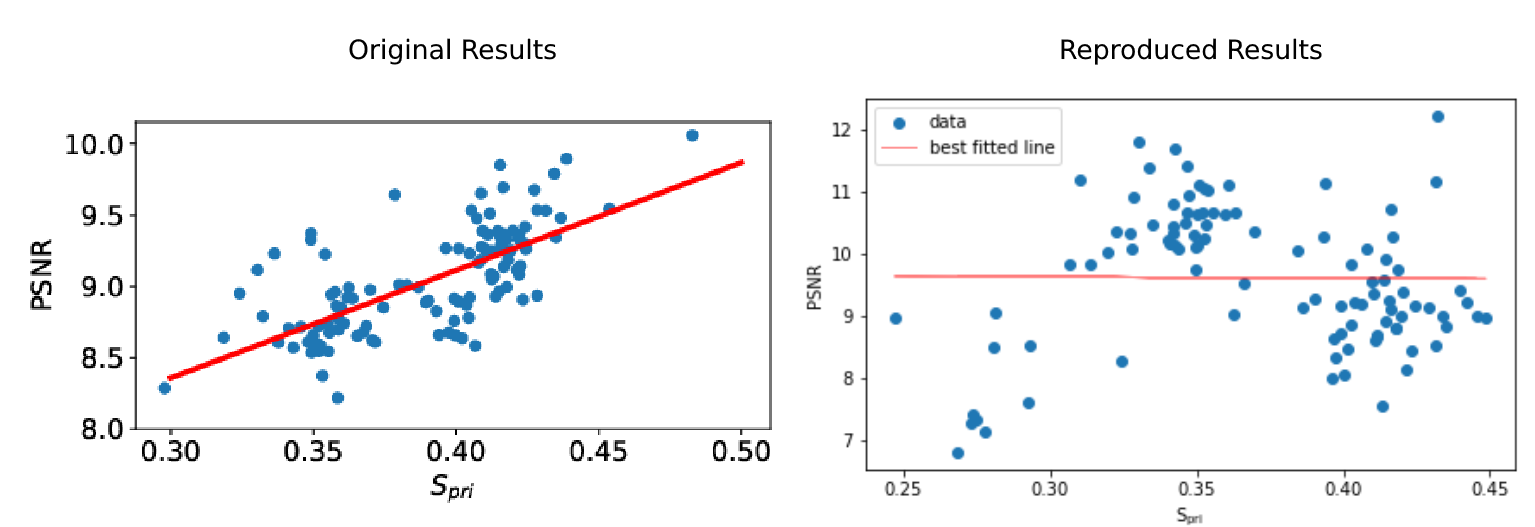
\includegraphics[width=12cm]{pics/correlation_comparison.png}
    \caption{Empirical validation of the correlation between the reconstruction (PSNR) score and the privacy score}
    \label{fig:correlation}
\end{figure}


\textbf{The Performance of Selected Policies} \citeauthor{gao2021privacy} claim the policies selected by the search algorithm reduce the PSNR reconstruction score significantly while not resulting in a great loss of accuracy. The results presented in the paper along with the results that resulted from the reproduction can be seen in Table \ref{tab:resls}.


Some results from the reproduction differ substantially from the ones presented in the paper, as can be seen from the red entries in Table \ref{tab:resls}. The biggest difference is the reconstruction score for the unaugmented policy of the Cifar100. Which differs greatly from the reconstruction score presented in the original paper. However, it is still significantly higher than that of the augmented policies.

The model's accuracies are comparable in most instances. But, the accuracy found in this research on the \textit{3-1-7} policy of the Cifar100 dataset scores almost 13\% below the accuracy of the unaugmented policy, compared to 6\% in the original paper.


% \begin{table}[h]\label{tab:resls}
% \begin{subtable}
% \begin{tabular}{l|l l l l}
%       \textbf{Policy} &  \textbf{Theirs} & \textbf{Ours} \\\hline
%   None &  &  &   \\
%   3-1-7 &  &  &  \\
%   43-18-18 &  &  & \\
%   Hybrid &  &  & \\
%   \hline
% \end{tabular}
% \caption{x}
% \end{subtable}
%\\
% \caption{Accuracies for cifar100}
% \end{table}


\begin{table}[h]
% 0.77007514 0.65832675 0.74841774 0.71064085
    \begin{subtable}{.50\linewidth}
        \centering
        {\begin{tabular}{|l|l l|}
             \hline
             \textbf{Policy} & \textbf{Theirs}   & \textbf{Ours}     \\\hline
             None            & 76.88             & 77.00             \\
             3-1-7           & \color{red} 70.56 & \color{red} 65.83 \\
             43-18-18        & 77.27             & 74.84             \\
             Hybrid          & \color{red} 77.92 & \color{red} 71.06 \\
             \hline
        \end{tabular}}
        \caption{Accuracy, Cifar100}\label{tab:1a}
    \end{subtable}%
    \hfill
    \begin{subtable}{.50\linewidth}
        \centering
        {\begin{tabular}{|l|l l |}
             \hline
             \textbf{Policy} & \textbf{Theirs}   & \textbf{Ours}              \\\hline
             None            & \color{red} 13.88 & \color{red} 9.94  $\pm 2.19$ \\
             3-1-7           & 6.58              & 6.28 $\pm 1.02$            \\
             43-18-18        & 8.56              & 8.71 $\pm 1.81 $           \\
             Hybrid          & 7.64              & 7.48  $\pm 1.85$             \\
             \hline
        \end{tabular}}
        \caption{PSNR, Cifar100}\label{tab:prs}
    \end{subtable}%
    \hfill
    \begin{subtable}{.50\linewidth}
        \centering
        {\begin{tabular}{|l|l l |}
             \hline
             \textbf{Policy} & \textbf{Theirs} & \textbf{Ours} \\\hline
             None            & 95.03           & 93.86         \\
             19-15-45        & 91.33           & 94.08         \\
             2-43-21         & 89.41           & 93.92         \\
             Hybrid          & 92.23           & 93.51         \\
             \hline
        \end{tabular}}
        \caption{Accuracy, F-Mnist}\label{tab:1b}
    \end{subtable}
    \hfill
    \begin{subtable}{.50\linewidth}
        \centering
        {\begin{tabular}{|l|l l|}
             \hline
             \textbf{Policy} & \textbf{Theirs}  & \textbf{Ours}               \\\hline
             None            & 10.04            & 9.71 $\pm 2.38$             \\
             19-15-45        & \color{red} 7.01 & \color{red}  9.88  $\pm 1.80$   \\
             2-43-21         & 7.75             & 7.94 $\pm  1.30$              \\
             Hybrid          & \color{red} 7.60 & \color{red} 8.94 $\pm 1.71$ \\
             \hline
        \end{tabular}}
        \caption{PSNR, F-Mnist}\label{tab:psnrs}
    \end{subtable}

    \caption{Comparison between model accuracies, in percentages (a), (c). Comparison between reconstruction scores, in decibels (b), (d). Results that differ substantially are highlighted (accuracy $\Delta 4\%$, PSNR $\Delta 2$dB). The \textit{None} policy performs no augmentations at all, and the \textit{Hybrid} policy randomly choses one of the augmented policies at random, for each image. Standard deviations are given for our PSNR scores ($\pm \sigma$).
    }
    \label{tab:resls}
\end{table}

Figure \ref{fig:imgs} shows a selection of image reconstructions performed by the attack model. Full sets of examples used to calculate the reconstructions scores can be found in Appendix \ref{apx:rdaa}.

\begingroup
\setlength{\tabcolsep}{2pt}
\begin{figure}[h]
    \captionsetup{justification=centering}
    \begin{subtable}{.25\linewidth}
        \centering
        {\begin{tabular}{ l l l l }
             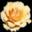
\includegraphics[width = 24pt]{repimages/ori_21_unaugmented.jpg} & 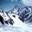
\includegraphics[width = 24pt]{repimages/ori_22_unaugmented.jpg}  & \includegraphics[width = 24pt]{repimages/ori_98_unaugmented.jpg} \\
             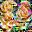
\includegraphics[width = 24pt]{repimages/rec_21_unaugmented.jpg} & 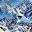
\includegraphics[width = 24pt]{repimages/rec_22_unaugmented.jpg}  & 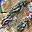
\includegraphics[width = 24pt]{repimages/rec_98_unaugmented.jpg}  &   \\
        \end{tabular}}
        \caption{Unaugmented, \\ Cifar100}%\label{tab:1a}
    \end{subtable}%
    \hfill
    \begin{subtable}{.25\linewidth}
        \centering
        {\begin{tabular}{ l l l l }
             \includegraphics[width = 24pt]{repimages/ori_21_hybrid.jpg} & \includegraphics[width = 24pt]{repimages/ori_22_hybrid.jpg}  & 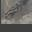
\includegraphics[width = 24pt]{repimages/ori_98_hybrid.jpg} \\
             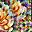
\includegraphics[width = 24pt]{repimages/rec_21_hybrid.jpg} & 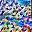
\includegraphics[width = 24pt]{repimages/rec_22_hybrid.jpg}  & 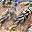
\includegraphics[width = 24pt]{repimages/rec_98_hybrid.jpg}  &   \\
        \end{tabular}}
        \caption{Hybrid, \\ Cifar100}%\label{tab:1a}
    \end{subtable}%
    \hfill
    \begin{subtable}{.25\linewidth}
        \centering
        {\begin{tabular}{ l l l l }
             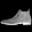
\includegraphics[width = 24pt]{repimages_fmnist/ori_1_unaug.jpg} & 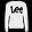
\includegraphics[width = 24pt]{repimages_fmnist/ori_2_unaug.jpg}  & \includegraphics[width = 24pt]{repimages_fmnist/ori_3_unaug.jpg} \\
             \includegraphics[width = 24pt]{repimages_fmnist/rec_1_unaug.jpg} & \includegraphics[width = 24pt]{repimages_fmnist/rec_2_unaug.jpg}  & 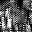
\includegraphics[width = 24pt]{repimages_fmnist/rec_3_unaug.jpg}  &   \\
        \end{tabular}}
        \caption{Unaugmented, \\ F-Mnist}%\label{tab:1a}
    \end{subtable}%
    \hfill
    \begin{subtable}{.25\linewidth}
        \centering
        {\begin{tabular}{ l l l l }
             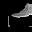
\includegraphics[width = 24pt]{repimages_fmnist/ori_1_hybrid.jpg} & \includegraphics[width = 24pt]{repimages_fmnist/ori_2_hybrid.jpg}  & \includegraphics[width = 24pt]{repimages_fmnist/ori_3_hybrid.jpg} \\
             \includegraphics[width = 24pt]{repimages_fmnist/rec_1_hybrid.jpg} & \includegraphics[width = 24pt]{repimages_fmnist/rec_2_hybrid.jpg}  & 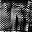
\includegraphics[width = 24pt]{repimages_fmnist/rec_3_hybrid.jpg}  &   \\
        \end{tabular}}
        \caption{Hybrid, \\ F-Mnist}%\label{tab:1a}
    \end{subtable}%
    \caption{ Original, augmented and reconstructed images. The images in the first row are either the original images for the unaugmented policy, or the augmented images for the hybrid policy. The images on the second row are the respective reconstructions found by the attack model.}
    \label{fig:imgs}
\end{figure}
\endgroup

% It can be seen from table \ref{tab:resls} that the obtained results form our reproductions differ from the results of the original paper. These are highlighted in the table with red colors to indicate substential differences. It can be seen that the accuracy of the hybrid augmentations from the reproduction are lower than the obtained accuracy from the orginal authors. The other differences are mainly in the PSNR score, where the fmnist dataset scores higher than the authors of the original paper claim, which indicate a smaller privacy score and thus results in the used data being easier to reproduce. 

\subsection{Additional Insight}
\textbf{Attacking with knowledge of policy.}
%A comparison of between the reconstruction with and without knowledge about the best policy can be found in Figure \ref{fig:attack}. It can be seen that the policies no longer score better than no policy. Crazy, right? Yes.
Comparisons between the default attack algorithm used in the original paper and the enhanced attack algorithm, which takes knowledge of the policy into account, are shown in Table \ref{tab:psnrdefenh} and Figure \ref{fig:attack}. It can be seen that the enhanced algorithm performs considerably better for all tested policies, and it even surpasses the reconstruction score of the unaugmented policy for the \textit{43-18-18} policy. More reconstruction examples can be seen in Appendix \ref{apx:reaa}.

% \begin{table}[htp]
% \centering
% \begin{tabular}{|l|ll|}
% \hline
% % Aligned is isolated_area
% \textbf{Policy} & \textbf{Default} & \textbf{Enhanced} \\ \hline
% None            &             9.94                   &  n/a                                    \\
% 3-1-7           &             6.28                   &      9.43                                \\ 
% 43-18-18   (preliminair!)   &       8.71                         &  10.34                     \\
% Hybrid          &             7.48                   &         9.42                        \\ \hline
% \end{tabular}
% \caption{PSNR of original attack model vs new attack model}
% \label{tab:attack}
% \end{table}

\begin{table}[h]
%    \begin{subtable}{1.0\linewidth}
        \centering
        \begin{tabular}{|l|ll|}
            \hline
% Aligned is isolated_area
            \textbf{Policy} & \textbf{Default} & \textbf{Enhanced} \\ \hline
            None            & 9.94             & n/a               \\
            3-1-7           & 6.28             & 9.43 $\pm 2.86$   \\
            43-18-18        & 8.71             & 10.34      $\pm 2.28$   \\
            Hybrid          & 7.48             & 9.42   $\pm 2.85$    \\ \hline

        \end{tabular}\\
        \vspace{7pt}
        \footnotesize {PSNR, Cifar100}
%    \end{subtable}%
    \caption{ Comparison between reconstruction scores of the default and enhanced algorithms, in decibels. Standard deviations are given for the enhanced PSNR scores ($\pm \sigma$). }\label{tab:erpsnr}
    \label{tab:psnrdefenh}
\end{table}

\begin{figure}[h]
%    \hfill
%    \\\\
    \begingroup
    \setlength{\tabcolsep}{1.8pt}
    \begin{subtable}{.33\linewidth}
        \centering
        {\begin{tabular}{ l l l }
%   \textbf{In} & \textbf{In*} & & \textbf{Out} & \textbf{Out*} & & \textbf{Paper} \\
             \includegraphics[width = 24pt]{enhimages317/ori_77.jpg} & 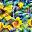
\includegraphics[width = 24pt]{defimages317/rec_77.jpg} &
             \includegraphics[width = 24pt]{enhimages317/rec_77.jpg} \\
             \includegraphics[width = 24pt]{enhimages317/ori_91.jpg} & \includegraphics[width = 24pt]{defimages317/rec_91.jpg} &
             \includegraphics[width = 24pt]{enhimages317/rec_91.jpg} \\
%   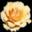
\includegraphics[width = 24pt]{repimages/ori_21_unaugmented.jpg} &  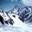
\includegraphics[width = 24pt]{repimages/ori_22_unaugmented.jpg} & &
%   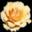
\includegraphics[width = 24pt]{repimages/ori_21_unaugmented.jpg} &  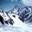
\includegraphics[width = 24pt]{repimages/ori_22_unaugmented.jpg} & &
%     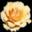
\includegraphics[width = 24pt]{repimages/ori_21_unaugmented.jpg} \\
        \end{tabular}}
        \caption{3-1-7}%\label{tab:1a}
    \end{subtable}%
%    \hfill
    \begin{subtable}{.33\linewidth}
        \centering
        {\begin{tabular}{ l l l }
%   \textbf{In} & \textbf{In*} & & \textbf{Out} & \textbf{Out*} & & \textbf{Paper} \\
             \includegraphics[width = 24pt]{enhimages431818/ori_77.jpg} & \includegraphics[width = 24pt]{defimages431818/rec_77.jpg} &
             \includegraphics[width = 24pt]{enhimages431818/rec_77.jpg} \\
             \includegraphics[width = 24pt]{enhimages431818/ori_91.jpg} & \includegraphics[width = 24pt]{defimages431818/rec_91.jpg} &
             \includegraphics[width = 24pt]{enhimages431818/rec_91.jpg} \\
%   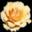
\includegraphics[width = 24pt]{repimages/ori_21_unaugmented.jpg} &  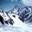
\includegraphics[width = 24pt]{repimages/ori_22_unaugmented.jpg} & &
%   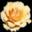
\includegraphics[width = 24pt]{repimages/ori_21_unaugmented.jpg} &  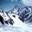
\includegraphics[width = 24pt]{repimages/ori_22_unaugmented.jpg} & &
%     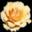
\includegraphics[width = 24pt]{repimages/ori_21_unaugmented.jpg} \\
        \end{tabular}}
        \caption{43-18-18}%\label{tab:1a}
    \end{subtable}%
%    \hfill
    \begin{subtable}{.33\linewidth}
        \centering
        {\begin{tabular}{ l l l }
%   \textbf{In} & \textbf{In*} & & \textbf{Out} & \textbf{Out*} & & \textbf{Paper} \\
             \includegraphics[width = 24pt]{enhimagesHybrid/ori_77.jpg} & \includegraphics[width = 24pt]{defimagesHybrid/rec_77.jpg} &
             \includegraphics[width = 24pt]{enhimagesHybrid/rec_77.jpg} \\
             \includegraphics[width = 24pt]{enhimagesHybrid/ori_91.jpg} & \includegraphics[width = 24pt]{defimagesHybrid/rec_91.jpg} &
             \includegraphics[width = 24pt]{enhimagesHybrid/rec_91.jpg} \\
%   \includegraphics[width = 25px]{repimages/ori_21_unaugmented.jpg} &  \includegraphics[width = 25px]{repimages/ori_22_unaugmented.jpg} & &
%   \includegraphics[width = 25px]{repimages/ori_21_unaugmented.jpg} &  \includegraphics[width = 25px]{repimages/ori_22_unaugmented.jpg} & &
%     \includegraphics[width = 25px]{repimages/ori_21_unaugmented.jpg} \\
        \end{tabular}}
        \caption{Hybrid}%\label{tab:1a}
    \end{subtable}%
    \endgroup
    \caption{Comparison between reconstructions of the default and enhanced algorithms. Column 1 of (a, b, c) are images augmented by the policy. Column 2 of (a, b, c) are the reconstructions given by the default algorithm. Column 3 of (a, b, c) are the reconstructions from the enhanced algorithm. }
    \label{fig:attack}
\end{figure}

\textbf{Diversity of policies}
In the original paper a brief analysis is provided of the privacy scores that the 50 augmentations achieve individually. The reproduced results can be seen in Figure \ref{fig:individual}. The results closely match the results in the original paper. The 10 best performing augmentations mostly overlap.

\begin{figure}[htp]
    \centering
    \includegraphics[width=8cm]{pics/policy_reconstruction_individual_fixed.png}
    \caption{Reconstruction score of the 50 augmentations when evaluated individually. A lower score is better. Top 5 of original authors marked in red.}
    \label{fig:individual}
\end{figure}

In the paper the authors state that the best performing augmentations are often selected in the best policies. To get more insight into this claim, 1500 random policies are evaluated in this research. The results can be seen in Figure \ref{fig:bunch_a_policies}. In this research the evaluation set was generated without a policy. It can be seen that most random policies score worse than this benchmark. More specifically, no-policy scored 0.32 on the privacy score while random policies scored 0.38 on average. Policies containing at least 2 of the top 10 individually scoring augmentations do scored slightly better with a score of 0.31. Policies consisting out of three of the top 5 policies scored better on average than 97.3\% of all policies tested.

\begin{figure}[htp]
    \centering
    \includegraphics[width=12cm]{pics/policy_comparison.png}
    \caption{Performance in the search algorithm benchmarks of 1500 random policies. Proposed Accuracy Score Threshold by original authors marked with dashed line. For the privacy score Split based on if they contain at least 2 of the top 10 policies (the policies with indices: 3, 15, 1, 26, 12, 43, 25, 13, 4 and 39)}
    \label{fig:bunch_a_policies}
\end{figure}

\newpage


\section{Discussion}\label{sec:discuss}
% Give your judgement on if your experimental results support the claims of the paper. Discuss the strengths and weaknesses of your approach - perhaps you didn't have time to run all the experiments, or perhaps you did additional experiments that further strengthened the claims in the paper.

The first claim, which states that the privacy score proposed in the paper correlates with the PSNR of a reconstruction attack, cannot be supported by the reproductions, since no correlation between the reconstruction PSNR and the privacy score has been found, as can be seen in figure \ref{fig:correlation}. A possible explanation for this could be that the model was trained with unaugmented data instead of augmented data, as the authors of the paper did not specify what was used to obtain the results. Due to computational constraints, it was not feasible to train the model on the complete dataset for every policy. For that reason the decision was made to evaluate the reconstructions attack for every policy using a model trained on unaugmented data. Further experimentations could be done to see if the pattern changes if this extensive test is done. A second difference between the experiments is that due to the limitations, the attack was only tested on 20 images instead of 100. This could make the results more uncertain, as a smaller sample size is used.

However, the second claim, stating that the policies selected by the search algorithm reduce the PSNR reconstruction score significantly while not resulting in a great loss of accuracy, holds true in the reproductions for almost all the selected policies. Nevertheless, the accuracy of the 3-1-7 policy is significantly lower when compared to the unaugmented policy, as can be seen in Table \ref{tab:1a}. There is no obvious explanation for this difference, but could be attributed to the non-deterministic nature of the training process of the model.

The results also hint that the protection provided by candidate policies can be circumvented by incorporating a translation module into the attack algorithm. In fact, it is possible that the augmented images are easier to reconstruct than the originals in this scenario. This can be seen from the PSNR score of the \textit{48-18-18} policy in Table \ref{tab:erpsnr}, as this score was higher than that of the unaugmented policy. A reason for this being the case could be the smaller search space for the attacker,
% Since it no longer has to reconstruct $N\times M\times 3$ individual pixels for a $N \times M$ image but, for example, if the augmented image is half the size, it only needs to reconstruct $\frac12 N\times M \times 3$ pixels in addition to the translation parameters $t_x$ and $t_y$.
as the default algorithm has to reconstruct a whole image consisting of $N\times M\times 3$ individual pixels for a $N \times M$ colour image, but the enhanced attack algorithm, thanks to its parameterization, only needs to reconstruct the non-black pixels and the translation parameters. For the \textit{3-1-7} policy for example, since roughly half the image is shifted outside the frame by the augmentations,
% which according to these policies are equal to a translational shift and colour adaptations that are equivalent to an image half the size,
the algorithm only needs to learn $\frac12 N\times M \times 3$ pixel values and the translation parameters $t_x$ and $t_y$.

The enhanced algorithm still cannot recover information from images that was deleted by the augmentations, such as the regions of the image that are cropped out, or the precise brightness, provided that the image is not augmented differently multiple times when used for collaborative training. This could prove useful in the future for protecting the privacy of participants in collaborative learning systems.
% But some of these aspects may still be recoverable if the image is augmented multiple times differently during the training of a model, as is standard practice when training neural networks.

\subsection{What Was Easy}
%  your judgement of what was easy to reproduce. Perhaps the author's code is clearly written and easy to run, so it was easy to verify the majority of original claims. Or, the explanation in the paper was really easy to follow and put into code. 
% Be careful not to give sweeping generalizations. Something that is easy for you might be difficult to others. Put what was easy in context and explain why it was easy (e.g. code had extensive API documentation and a lot of examples that matched experiments in papers). 
The design of the search algorithm allowed for easy iterations of experiments since obtaining the scores of a single policy can be done in under a minute. This enabled us to test a lot of policies in different scenario's which gave a lot of insight into the distribution of the performance of augmentations. Well-performing policies can often be found within an hour.

\subsection{What Was Difficult}
% List part of the reproduction study that took more time than you anticipated or you felt were difficult. 
% Be careful to put your discussion in context. For example, don't say "the maths was difficult to follow", say "the math requires advanced knowledge of calculus to follow". 

To obtain the PSNR and accuracy score of a policy, the architecture needs to be trained for about 10 GPU-hours. This makes it difficult to verify how well the search metrics correlate with these scores. It also prevented us to test the random policy baseline, as this requires the training to be repeated at least 10 times which requires significant computational power.

\subsection{Communication With Original Authors}
% Document the extent of (or lack of) communication with the original authors. To make sure the reproducibility report is a fair assessment of the original research we recommend getting in touch with the original authors. You can ask authors specific questions, or if you don't have any questions you can send them the full report to get their feedback before it gets published. 
An e-mail was sent to the original authors regarding the differing results in the first claim and for the mathematical intuition behind the accuracy score. Unfortunately no response has been received so far.
